% Generated by make_fig_tool.py from programs/ansatz.py, srcML and the tool. Do not edit by hand.
\documentclass[tikz,border=2pt]{standalone}
\usepackage[T1]{fontenc}
\usepackage{newtxtext,newtxmath}
\usepackage[varqu,scaled=0.95]{zi4}
\usetikzlibrary{arrows.meta,calc}
\definecolor{ink}{HTML}{1F2328}\definecolor{mute}{HTML}{6E7781}\definecolor{rule}{HTML}{D0D7DE}
\definecolor{wire}{HTML}{0969DA}\definecolor{wireL}{HTML}{DDEBFF}\definecolor{tree}{HTML}{6639BA}
\definecolor{hlC}{HTML}{FFF1B8}
\newcommand{\hlbox}[1]{{\setlength{\fboxsep}{0.4pt}\colorbox{hlC}{\strut #1}}}
\newcommand{\hlm}[1]{\raisebox{0.9ex}{\textcolor{tree}{\fontsize{5.4}{6}\selectfont\bfseries\rmfamily #1}}}
\newcommand{\hl}[1]{\textcolor{tree}{\bfseries #1}}
\tikzset{
  >={Stealth[length=3.6pt,width=3.2pt]},
  stage/.style={font=\footnotesize\bfseries, text=ink, anchor=west, inner sep=0pt},
  stnum/.style={circle, draw=ink, line width=0.6pt, font=\scriptsize\bfseries, text=ink, inner sep=0pt, minimum size=9pt},
  xml/.style={font=\ttfamily\fontsize{5.9}{6.6}\selectfont, anchor=west, inner sep=0pt},
  note/.style={font=\fontsize{6.2}{7.4}\selectfont\itshape, execute at begin node={\hyphenpenalty=10000}, text=mute, inner sep=0pt},
  flowarrow/.style={->, line width=0.7pt, draw=ink},
}
\begin{document}
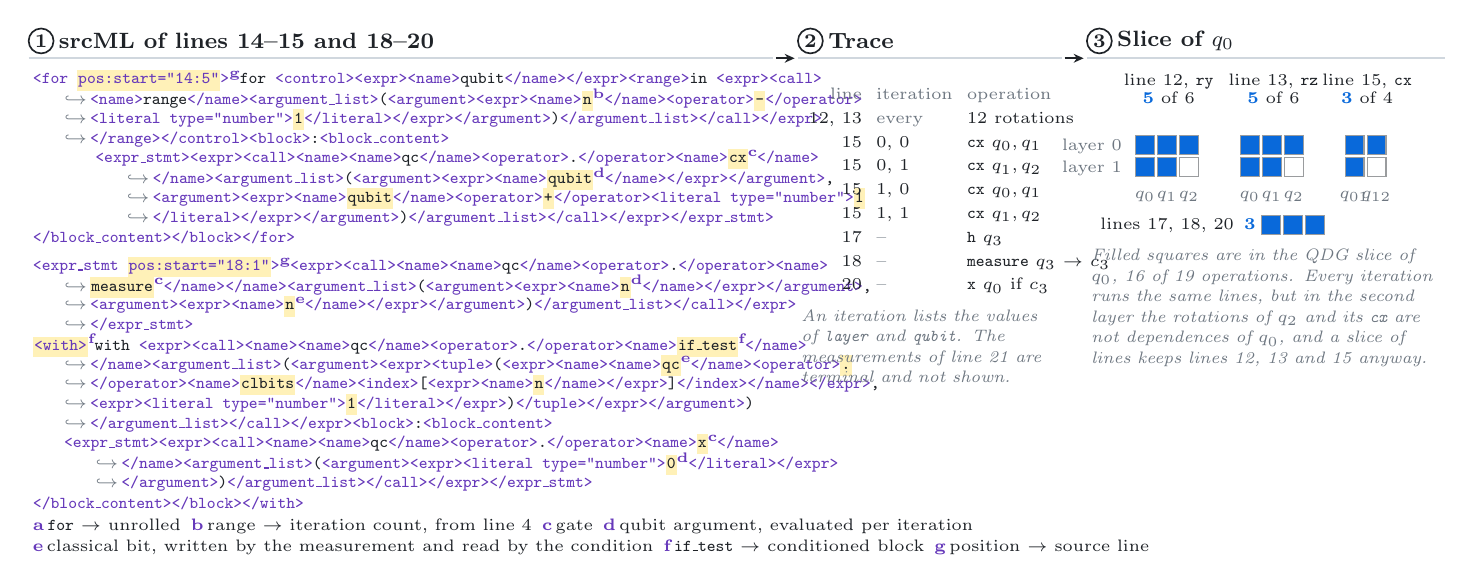
\begin{tikzpicture}

\node[stnum] at (0.16,0.5) {1};
\node[stage] at (0.38,0.5) {srcML of lines 14--15 and 18--20};
\draw[rule, line width=0.6pt] (0,0.28) -- (9.45,0.28);
\node[xml] at (0.05,0.0) {\textcolor{tree}{<for \hlbox{pos:start="14:5"}>}\hlm{g}\textcolor{ink}{\bfseries for }\textcolor{tree}{<control>}\textcolor{tree}{<expr>}\textcolor{tree}{<name>}\textcolor{ink}{\bfseries qubit}\textcolor{tree}{</name>}\textcolor{tree}{</expr>}\textcolor{ink}{\bfseries  }\textcolor{tree}{<range>}\textcolor{ink}{\bfseries in }\textcolor{tree}{<expr>}\textcolor{tree}{<call>}};
\node[xml] at (0.446,-0.25) {\textcolor{mute}{\rmfamily\fontsize{5.6}{6}\selectfont$\hookrightarrow$}\,\textcolor{tree}{<name>}\textcolor{ink}{\bfseries range}\textcolor{tree}{</name>}\textcolor{tree}{<argument\_list>}\textcolor{ink}{\bfseries (}\textcolor{tree}{<argument>}\textcolor{tree}{<expr>}\textcolor{tree}{<name>}\hlbox{\textcolor{ink}{\bfseries n}}\hlm{b}\textcolor{tree}{</name>}\textcolor{ink}{\bfseries  }\textcolor{tree}{<operator>}\hlbox{\textcolor{ink}{\bfseries -}}\textcolor{tree}{</operator>}\textcolor{ink}{\bfseries  }};
\node[xml] at (0.446,-0.5) {\textcolor{mute}{\rmfamily\fontsize{5.6}{6}\selectfont$\hookrightarrow$}\,\textcolor{tree}{<literal type="number">}\hlbox{\textcolor{ink}{\bfseries 1}}\textcolor{tree}{</literal>}\textcolor{tree}{</expr>}\textcolor{tree}{</argument>}\textcolor{ink}{\bfseries )}\textcolor{tree}{</argument\_list>}\textcolor{tree}{</call>}\textcolor{tree}{</expr>}};
\node[xml] at (0.446,-0.75) {\textcolor{mute}{\rmfamily\fontsize{5.6}{6}\selectfont$\hookrightarrow$}\,\textcolor{tree}{</range>}\textcolor{tree}{</control>}\textcolor{tree}{<block>}\textcolor{ink}{\bfseries :}\textcolor{tree}{<block\_content>}};
\node[xml] at (0.8420000000000001,-1.0) {\textcolor{tree}{<expr\_stmt>}\textcolor{tree}{<expr>}\textcolor{tree}{<call>}\textcolor{tree}{<name>}\textcolor{tree}{<name>}\textcolor{ink}{\bfseries qc}\textcolor{tree}{</name>}\textcolor{tree}{<operator>}\textcolor{ink}{\bfseries .}\textcolor{tree}{</operator>}\textcolor{tree}{<name>}\hlbox{\textcolor{ink}{\bfseries cx}}\hlm{c}\textcolor{tree}{</name>}};
\node[xml] at (1.2380000000000002,-1.25) {\textcolor{mute}{\rmfamily\fontsize{5.6}{6}\selectfont$\hookrightarrow$}\,\textcolor{tree}{</name>}\textcolor{tree}{<argument\_list>}\textcolor{ink}{\bfseries (}\textcolor{tree}{<argument>}\textcolor{tree}{<expr>}\textcolor{tree}{<name>}\hlbox{\textcolor{ink}{\bfseries qubit}}\hlm{d}\textcolor{tree}{</name>}\textcolor{tree}{</expr>}\textcolor{tree}{</argument>}\textcolor{ink}{\bfseries , }};
\node[xml] at (1.2380000000000002,-1.5) {\textcolor{mute}{\rmfamily\fontsize{5.6}{6}\selectfont$\hookrightarrow$}\,\textcolor{tree}{<argument>}\textcolor{tree}{<expr>}\textcolor{tree}{<name>}\hlbox{\textcolor{ink}{\bfseries qubit}}\textcolor{tree}{</name>}\textcolor{ink}{\bfseries  }\textcolor{tree}{<operator>}\hlbox{\textcolor{ink}{\bfseries +}}\textcolor{tree}{</operator>}\textcolor{ink}{\bfseries  }\textcolor{tree}{<literal type="number">}\hlbox{\textcolor{ink}{\bfseries 1}}};
\node[xml] at (1.2380000000000002,-1.75) {\textcolor{mute}{\rmfamily\fontsize{5.6}{6}\selectfont$\hookrightarrow$}\,\textcolor{tree}{</literal>}\textcolor{tree}{</expr>}\textcolor{tree}{</argument>}\textcolor{ink}{\bfseries )}\textcolor{tree}{</argument\_list>}\textcolor{tree}{</call>}\textcolor{tree}{</expr>}\textcolor{tree}{</expr\_stmt>}};
\node[xml] at (0.05,-2.0) {\textcolor{tree}{</block\_content>}\textcolor{tree}{</block>}\textcolor{tree}{</for>}};
\node[xml] at (0.05,-2.37) {\textcolor{tree}{<expr\_stmt \hlbox{pos:start="18:1"}>}\hlm{g}\textcolor{tree}{<expr>}\textcolor{tree}{<call>}\textcolor{tree}{<name>}\textcolor{tree}{<name>}\textcolor{ink}{\bfseries qc}\textcolor{tree}{</name>}\textcolor{tree}{<operator>}\textcolor{ink}{\bfseries .}\textcolor{tree}{</operator>}\textcolor{tree}{<name>}};
\node[xml] at (0.446,-2.62) {\textcolor{mute}{\rmfamily\fontsize{5.6}{6}\selectfont$\hookrightarrow$}\,\hlbox{\textcolor{ink}{\bfseries measure}}\hlm{c}\textcolor{tree}{</name>}\textcolor{tree}{</name>}\textcolor{tree}{<argument\_list>}\textcolor{ink}{\bfseries (}\textcolor{tree}{<argument>}\textcolor{tree}{<expr>}\textcolor{tree}{<name>}\hlbox{\textcolor{ink}{\bfseries n}}\hlm{d}\textcolor{tree}{</name>}\textcolor{tree}{</expr>}\textcolor{tree}{</argument>}\textcolor{ink}{\bfseries , }};
\node[xml] at (0.446,-2.87) {\textcolor{mute}{\rmfamily\fontsize{5.6}{6}\selectfont$\hookrightarrow$}\,\textcolor{tree}{<argument>}\textcolor{tree}{<expr>}\textcolor{tree}{<name>}\hlbox{\textcolor{ink}{\bfseries n}}\hlm{e}\textcolor{tree}{</name>}\textcolor{tree}{</expr>}\textcolor{tree}{</argument>}\textcolor{ink}{\bfseries )}\textcolor{tree}{</argument\_list>}\textcolor{tree}{</call>}\textcolor{tree}{</expr>}};
\node[xml] at (0.446,-3.12) {\textcolor{mute}{\rmfamily\fontsize{5.6}{6}\selectfont$\hookrightarrow$}\,\textcolor{tree}{</expr\_stmt>}};
\node[xml] at (0.05,-3.37) {\hlbox{\textcolor{tree}{<with>}}\hlm{f}\textcolor{ink}{\bfseries with }\textcolor{tree}{<expr>}\textcolor{tree}{<call>}\textcolor{tree}{<name>}\textcolor{tree}{<name>}\textcolor{ink}{\bfseries qc}\textcolor{tree}{</name>}\textcolor{tree}{<operator>}\textcolor{ink}{\bfseries .}\textcolor{tree}{</operator>}\textcolor{tree}{<name>}\hlbox{\textcolor{ink}{\bfseries if\_test}}\hlm{f}\textcolor{tree}{</name>}};
\node[xml] at (0.446,-3.62) {\textcolor{mute}{\rmfamily\fontsize{5.6}{6}\selectfont$\hookrightarrow$}\,\textcolor{tree}{</name>}\textcolor{tree}{<argument\_list>}\textcolor{ink}{\bfseries (}\textcolor{tree}{<argument>}\textcolor{tree}{<expr>}\textcolor{tree}{<tuple>}\textcolor{ink}{\bfseries (}\textcolor{tree}{<expr>}\textcolor{tree}{<name>}\textcolor{tree}{<name>}\hlbox{\textcolor{ink}{\bfseries qc}}\hlm{e}\textcolor{tree}{</name>}\textcolor{tree}{<operator>}\hlbox{\textcolor{ink}{\bfseries .}}};
\node[xml] at (0.446,-3.87) {\textcolor{mute}{\rmfamily\fontsize{5.6}{6}\selectfont$\hookrightarrow$}\,\textcolor{tree}{</operator>}\textcolor{tree}{<name>}\hlbox{\textcolor{ink}{\bfseries clbits}}\textcolor{tree}{</name>}\textcolor{tree}{<index>}\textcolor{ink}{\bfseries [}\textcolor{tree}{<expr>}\textcolor{tree}{<name>}\hlbox{\textcolor{ink}{\bfseries n}}\textcolor{tree}{</name>}\textcolor{tree}{</expr>}\textcolor{ink}{\bfseries ]}\textcolor{tree}{</index>}\textcolor{tree}{</name>}\textcolor{tree}{</expr>}\textcolor{ink}{\bfseries , }};
\node[xml] at (0.446,-4.12) {\textcolor{mute}{\rmfamily\fontsize{5.6}{6}\selectfont$\hookrightarrow$}\,\textcolor{tree}{<expr>}\textcolor{tree}{<literal type="number">}\hlbox{\textcolor{ink}{\bfseries 1}}\textcolor{tree}{</literal>}\textcolor{tree}{</expr>}\textcolor{ink}{\bfseries )}\textcolor{tree}{</tuple>}\textcolor{tree}{</expr>}\textcolor{tree}{</argument>}\textcolor{ink}{\bfseries )}};
\node[xml] at (0.446,-4.37) {\textcolor{mute}{\rmfamily\fontsize{5.6}{6}\selectfont$\hookrightarrow$}\,\textcolor{tree}{</argument\_list>}\textcolor{tree}{</call>}\textcolor{tree}{</expr>}\textcolor{tree}{<block>}\textcolor{ink}{\bfseries :}\textcolor{tree}{<block\_content>}};
\node[xml] at (0.446,-4.62) {\textcolor{tree}{<expr\_stmt>}\textcolor{tree}{<expr>}\textcolor{tree}{<call>}\textcolor{tree}{<name>}\textcolor{tree}{<name>}\textcolor{ink}{\bfseries qc}\textcolor{tree}{</name>}\textcolor{tree}{<operator>}\textcolor{ink}{\bfseries .}\textcolor{tree}{</operator>}\textcolor{tree}{<name>}\hlbox{\textcolor{ink}{\bfseries x}}\hlm{c}\textcolor{tree}{</name>}};
\node[xml] at (0.8420000000000001,-4.87) {\textcolor{mute}{\rmfamily\fontsize{5.6}{6}\selectfont$\hookrightarrow$}\,\textcolor{tree}{</name>}\textcolor{tree}{<argument\_list>}\textcolor{ink}{\bfseries (}\textcolor{tree}{<argument>}\textcolor{tree}{<expr>}\textcolor{tree}{<literal type="number">}\hlbox{\textcolor{ink}{\bfseries 0}}\hlm{d}\textcolor{tree}{</literal>}\textcolor{tree}{</expr>}};
\node[xml] at (0.8420000000000001,-5.12) {\textcolor{mute}{\rmfamily\fontsize{5.6}{6}\selectfont$\hookrightarrow$}\,\textcolor{tree}{</argument>}\textcolor{ink}{\bfseries )}\textcolor{tree}{</argument\_list>}\textcolor{tree}{</call>}\textcolor{tree}{</expr>}\textcolor{tree}{</expr\_stmt>}};
\node[xml] at (0.05,-5.37) {\textcolor{tree}{</block\_content>}\textcolor{tree}{</block>}\textcolor{tree}{</with>}};
\node[anchor=north west, align=left, font=\fontsize{6.2}{7.6}\selectfont, text=ink, inner sep=0pt] at (0.05,-5.5600000000000005) {\hl{a}\,\texttt{for} $\to$ unrolled\enspace \hl{b}\,range $\to$ iteration count, from line 4\enspace \hl{c}\,gate\enspace \hl{d}\,qubit argument, evaluated per iteration\\\hl{e}\,classical bit, written by the measurement and read by the condition\enspace \hl{f}\,\texttt{if\_test} $\to$ conditioned block\enspace \hl{g}\,position $\to$ source line};
\node[stnum] at (9.93,0.5) {2};
\node[stage] at (10.15,0.5) {Trace};
\draw[rule, line width=0.6pt] (9.77,0.28) -- (13.12,0.28);
\node[anchor=north west, font=\fontsize{6.4}{7.6}\selectfont, text=ink, inner sep=0pt] (trace) at (9.809999999999999,-0.05) {\setlength{\tabcolsep}{2.6pt}\begin{tabular}{rll}\textcolor{mute}{line}&\textcolor{mute}{iteration}&\textcolor{mute}{operation}\\[1pt]12, 13&\textcolor{mute}{every}&12 rotations\\[1pt]15&0, 0&\texttt{cx} $q_0$,\,$q_1$\\[1pt]15&0, 1&\texttt{cx} $q_1$,\,$q_2$\\[1pt]15&1, 0&\texttt{cx} $q_0$,\,$q_1$\\[1pt]15&1, 1&\texttt{cx} $q_1$,\,$q_2$\\[1pt]17&\textcolor{mute}{--}&\texttt{h} $q_3$\\[1pt]18&\textcolor{mute}{--}&\texttt{measure} $q_3$ $\to$ $c_{3}$\\[1pt]20&\textcolor{mute}{--}&\texttt{x} $q_0$ if $c_{3}$\\[1pt]\end{tabular}};
\node[note, anchor=north west, align=left, text width=3.25cm] at ($(trace.south west)+(0,-0.12)$) {An iteration lists the values of \texttt{layer} and \texttt{qubit}. The measurements of line 21 are terminal and not shown.};
\node[stnum] at (13.6,0.5) {3};
\node[stage] at (13.82,0.5) {Slice of $q_0$};
\draw[rule, line width=0.6pt] (13.44,0.28) -- (17.99,0.28);
\node[font=\fontsize{6.3}{7.4}\selectfont, text=ink, anchor=south, align=center] at (14.479999999999999,-0.42) {line 12, \texttt{ry}\\[-1pt]\textcolor{wire}{\bfseries 5} of 6};
\node[font=\fontsize{5.8}{6.5}\selectfont, text=mute, anchor=east] at (14.009999999999998,-0.84) {layer 0};
\draw[draw=ink!45, line width=0.4pt, fill=wire] (14.059999999999999,-0.7) rectangle ++(0.24000000000000002,-0.24000000000000002);
\draw[draw=ink!45, line width=0.4pt, fill=wire] (14.339999999999998,-0.7) rectangle ++(0.24000000000000002,-0.24000000000000002);
\draw[draw=ink!45, line width=0.4pt, fill=wire] (14.62,-0.7) rectangle ++(0.24000000000000002,-0.24000000000000002);
\node[font=\fontsize{5.8}{6.5}\selectfont, text=mute, anchor=east] at (14.009999999999998,-1.12) {layer 1};
\draw[draw=ink!45, line width=0.4pt, fill=wire] (14.059999999999999,-0.98) rectangle ++(0.24000000000000002,-0.24000000000000002);
\draw[draw=ink!45, line width=0.4pt, fill=wire] (14.339999999999998,-0.98) rectangle ++(0.24000000000000002,-0.24000000000000002);
\draw[draw=ink!45, line width=0.4pt, fill=white] (14.62,-0.98) rectangle ++(0.24000000000000002,-0.24000000000000002);
\node[font=\fontsize{5.6}{6}\selectfont, text=mute, anchor=north] at (14.179999999999998,-1.28) {$q_{0}$};
\node[font=\fontsize{5.6}{6}\selectfont, text=mute, anchor=north] at (14.459999999999997,-1.28) {$q_{1}$};
\node[font=\fontsize{5.6}{6}\selectfont, text=mute, anchor=north] at (14.739999999999998,-1.28) {$q_{2}$};
\node[font=\fontsize{6.3}{7.4}\selectfont, text=ink, anchor=south, align=center] at (15.809999999999999,-0.42) {line 13, \texttt{rz}\\[-1pt]\textcolor{wire}{\bfseries 5} of 6};
\draw[draw=ink!45, line width=0.4pt, fill=wire] (15.389999999999999,-0.7) rectangle ++(0.24000000000000002,-0.24000000000000002);
\draw[draw=ink!45, line width=0.4pt, fill=wire] (15.669999999999998,-0.7) rectangle ++(0.24000000000000002,-0.24000000000000002);
\draw[draw=ink!45, line width=0.4pt, fill=wire] (15.95,-0.7) rectangle ++(0.24000000000000002,-0.24000000000000002);
\draw[draw=ink!45, line width=0.4pt, fill=wire] (15.389999999999999,-0.98) rectangle ++(0.24000000000000002,-0.24000000000000002);
\draw[draw=ink!45, line width=0.4pt, fill=wire] (15.669999999999998,-0.98) rectangle ++(0.24000000000000002,-0.24000000000000002);
\draw[draw=ink!45, line width=0.4pt, fill=white] (15.95,-0.98) rectangle ++(0.24000000000000002,-0.24000000000000002);
\node[font=\fontsize{5.6}{6}\selectfont, text=mute, anchor=north] at (15.509999999999998,-1.28) {$q_{0}$};
\node[font=\fontsize{5.6}{6}\selectfont, text=mute, anchor=north] at (15.789999999999997,-1.28) {$q_{1}$};
\node[font=\fontsize{5.6}{6}\selectfont, text=mute, anchor=north] at (16.07,-1.28) {$q_{2}$};
\node[font=\fontsize{6.3}{7.4}\selectfont, text=ink, anchor=south, align=center] at (17.0,-0.42) {line 15, \texttt{cx}\\[-1pt]\textcolor{wire}{\bfseries 3} of 4};
\draw[draw=ink!45, line width=0.4pt, fill=wire] (16.72,-0.7) rectangle ++(0.24000000000000002,-0.24000000000000002);
\draw[draw=ink!45, line width=0.4pt, fill=wire] (17.0,-0.7) rectangle ++(0.24000000000000002,-0.24000000000000002);
\draw[draw=ink!45, line width=0.4pt, fill=wire] (16.72,-0.98) rectangle ++(0.24000000000000002,-0.24000000000000002);
\draw[draw=ink!45, line width=0.4pt, fill=white] (17.0,-0.98) rectangle ++(0.24000000000000002,-0.24000000000000002);
\node[font=\fontsize{5.6}{6}\selectfont, text=mute, anchor=north] at (16.84,-1.28) {$q_{01}$};
\node[font=\fontsize{5.6}{6}\selectfont, text=mute, anchor=north] at (17.12,-1.28) {$q_{12}$};
\node[font=\fontsize{6.3}{7.4}\selectfont, text=ink, anchor=west] at (13.49,-1.8399999999999999) {lines 17, 18, 20\enspace\textcolor{wire}{\bfseries 3} of 3};
\draw[draw=ink!45, line width=0.4pt, fill=wire] (15.655999999999999,-1.72) rectangle ++(0.24000000000000002,-0.24000000000000002);
\draw[draw=ink!45, line width=0.4pt, fill=wire] (15.935999999999998,-1.72) rectangle ++(0.24000000000000002,-0.24000000000000002);
\draw[draw=ink!45, line width=0.4pt, fill=wire] (16.215999999999998,-1.72) rectangle ++(0.24000000000000002,-0.24000000000000002);
\node[note, anchor=north west, align=left, text width=4.45cm] at (13.49,-2.14) {Filled squares are in the QDG slice of $q_0$, 16 of 19 operations. Every iteration runs the same lines, but in the second layer the rotations of $q_2$ and its \texttt{cx} are not dependences of $q_0$, and a slice of lines keeps lines 12, 13 and 15 anyway.};
\draw[flowarrow] (9.489999999999998,0.28) -- (9.73,0.28);
\draw[flowarrow] (13.159999999999998,0.28) -- (13.4,0.28);
\end{tikzpicture}
\end{document}
